\section{SVM}
Temel amacı, verileri bir hiperdüzlem üzerinde sınıflandırmak veya regresyon analizi yapmaktır.

\begin{figure}[h]
    \centering
    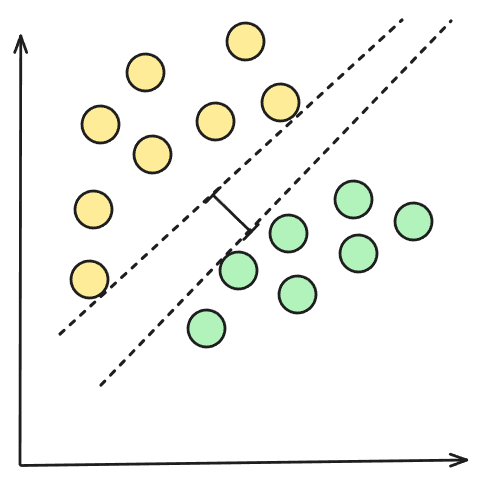
\includegraphics[width=1\textwidth]{images/svm.png}
    \caption{Destek vektör makineleri.}
    \label{fig:enter-label}
\end{figure}

\subsection{Çalışma Adımları}
SVM, bu hiperdüzlemi oluştururken, sınıflar arasındaki en büyük marjı (boşluk) bulmaya çalışır. Marj, hiperdüzleme en yakın veri noktalarından uzaklık olarak tanımlanır ve bu noktalara "destek vektörleri" denir. Hiperdüzlem, bu destek vektörleri arasında yer alır ve iki sınıf arasındaki boşluğu maksimize eder. SVM'nin çalışma prensibi matematiksel olarak iki sınıf için aşağıdaki şekilde ifade edilir:\\

Veri noktası: (x,y) Hiperdüzlem: w . x + b = 0
\begin{itemize}
    \item w: Hiperdüzlemi belirleyen normal vektör (ağırlıklar).
    \item x: Veri noktasının özellik vektörü.
    \item b: Bias terimi.
\end{itemize}

Sınıf tahminlemesi yapmak için, veri noktasını hiperdüzlem formülüne yerleştiririz:

\begin{itemize}
    \item Eğer w * x+b>0 ise, veri noktası sınıf +1'e aittir.
    \item Eğer w * x+b<0 ise, veri noktası sınıf -1'e aittir.
\end{itemize}

\subsection{Avantajları}
\begin{itemize}
    \item Etkili performans
    \item Hem sınıflandırma hem regresyon problemlerinde kullanılır.
\end{itemize}

\subsection{Dezavantajları}
\begin{itemize}
    \item Büyük veri kümelerinde eğitim süresi uzun olabilir.
    \item Çoklu sınıf, çoklu özellik sorunlarına karşı performansı düşebilir.
\end{itemize}

\subsection{Hiperparametreler}
\begin{table}[h]
\centering
{\scriptsize\renewcommand{\arraystretch}{0.4}
{\resizebox*{\linewidth}{0.5\textwidth}{
\begin{tabular}{|p{2cm}|p{1cm}|p{1cm}|p{7cm}|}
\hline
Parametre & Type & Default & Açıklama \\ \hline
C & float & 1 & C, SVM'nin bir hiperdüzlemi oluştururken ne kadar hata kabul edeceğinizi kontrol eden bir hiperparametredir. Küçük bir C değeri, daha geniş bir marj ve daha fazla eğim sağlar, ancak bazı veri noktalarının hatalı sınıflandırılmasına neden olabilir. Büyük bir C değeri, daha dar bir marj ve daha az hata kabul eder. C'nin değeri modelin aşırı uyuma (overfitting) karşı hassasiyetini etkiler. C değeri ne kadar büyükse, aşırı uyuma o kadar eğilimli olabilir. \\ \hline
kernel & "linear", "poly", "rbf", "sigmoid" & "rbf" & Çekirdek \\ \hline
gamma & "scale" ,"auto" & "scale" & Gamma, bir veri noktasının diğer veri noktalarına ne kadar etki etmesini kontrol eder. Küçük bir gamma değeri, uzak noktaların etkisinin büyük olmasını sağlar. Büyük bir gamma değeri ise yakın noktaların etkisinin büyük olmasını sağlar. \\ \hline
degree & int & 3 & Polinum çekirdek derecesi. Sadece kernel "poly" ise kullanılır. \\ \hline

\end{tabular}
}}}
\end{table}

\newpage